\clearpage
\subsection{Robustness}
\label{app:robustness}
Although current LMs perform remarkably well in the zero-shot setting, they are still known to be sensitive to the exact format of their prompt (see \citet{eval-harness,liang2022holistic,srivastava2022beyond} for extensive evaluations).
Thus, one might wonder: Are the distributions we are obtaining from LMs robust to such design choices?
Before we delve into this further, it is important to note that humans also exhibit a similar sensitivity.
In the context of Pew surveys, human respondents are also sensitive to factors such as option ordering and question formatting.
Nevertheless, we test how robust our analysis is to: (i) the order in which options for a question are presented to the model and (ii) prompt formatting.
Even though we see small fluctuations in the actual representativeness scores through these interventions, the overall trends remain unchanged---the relative ranking of models and the subgroups they tend to align with.




\subsubsection{Sensitivity to option ordering}

We exactly repeat our analysis from the main paper, but present the model with answer choices for a question in a randomly permuted (rather than the default ordinal) order. 
For instance, for the question in Figure~\ref{fig:prompt_example}, we might present the options as ``A: Not too much, B: A great deal, C: A fair amount, D: Not at all''.
For a given question, the same random permutation is used across LMs. 

Under such permutations, we see a small drop in the representativeness scores of all models.
We believe that this is at least partly because the reference human distribution is based on survey responses where humans were presented options in an ordinal manner rather than randomly.
Since humans are also sensitive to option ordering, we believe this has some effect on the observed human opinion distribution.
However, as mentioned above, the overall and subgroup-level trends remain largely consistent as seen from Figure~\ref{figapp:perm_alignment_basic}.

\begin{figure*}[!h]
    \caption{Effect of option ordering on overall and subgroup representativeness (continued on next pages).}
    \label{figapp:perm_alignment_basic}
    \vskip 0.2in
    \begin{subfigure}[b]{1\textwidth}
        \centering
        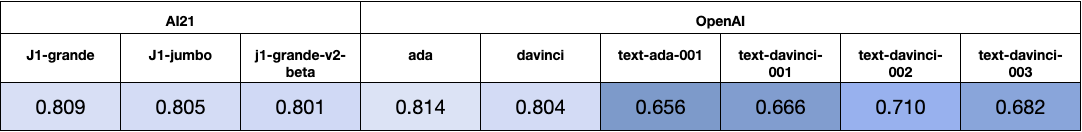
\includegraphics[width=1\columnwidth]{Figures/permuted_basic_alignment_table.png}
        \caption{Overall representativeness}
    \end{subfigure} 
    \begin{subfigure}[b]{1\textwidth}
        \centering
        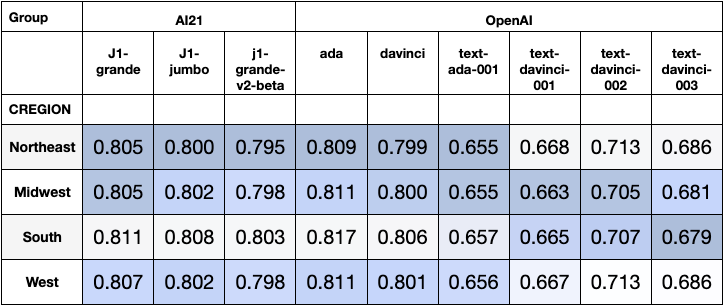
\includegraphics[width=0.55\columnwidth]{Figures/permuted_group_alignment_F_CREGION.png}
        \caption{Census region}
    \end{subfigure} 
    \begin{subfigure}[b]{1\textwidth}
        \centering
        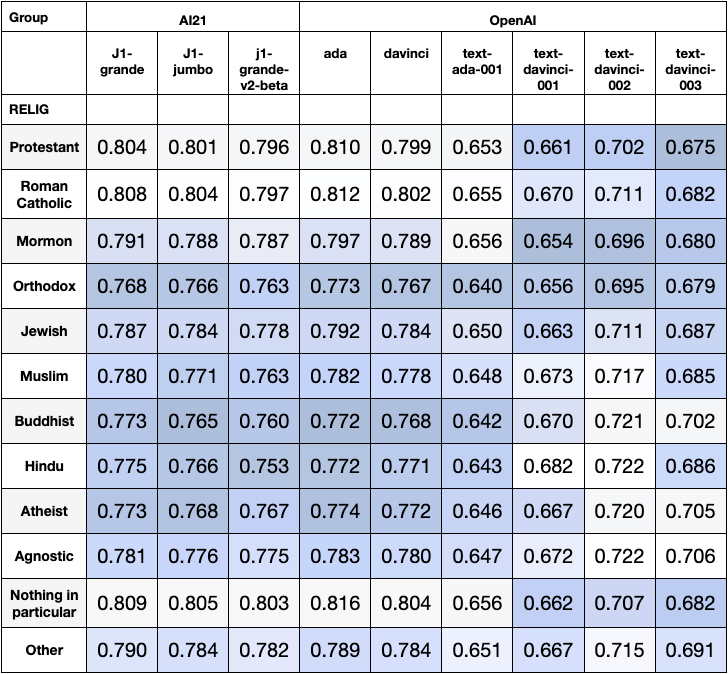
\includegraphics[width=0.55\columnwidth]{Figures/permuted_group_alignment_F_RELIG.png}
        \caption{Religious attendance}
    \end{subfigure} 
    \vskip -0.2in
\end{figure*}
\begin{figure*}[!h]
    \ContinuedFloat
    \vskip 0.2in
    \begin{subfigure}[b]{1\textwidth}
        \centering
        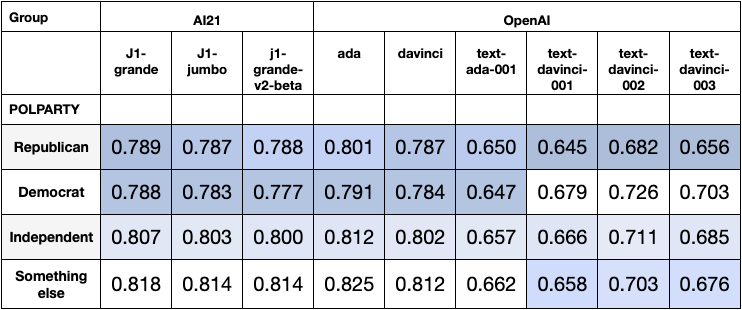
\includegraphics[width=0.45\columnwidth]{Figures/permuted_group_alignment_F_PARTY_FINAL.png}
        \caption{Political party affiliation}
    \end{subfigure} 
    \begin{subfigure}[b]{1\textwidth}
        \centering
        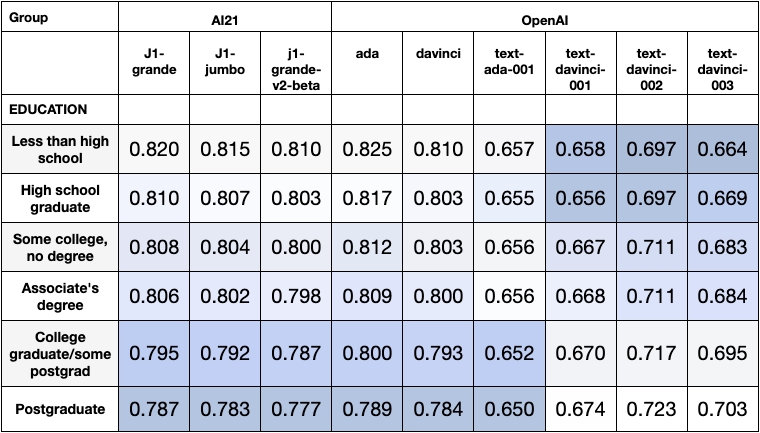
\includegraphics[width=0.45\columnwidth]{Figures/permuted_group_alignment_F_EDUCCAT2.png}
        \caption{Education}
    \end{subfigure}
    \begin{subfigure}[b]{1\textwidth}
        \centering
        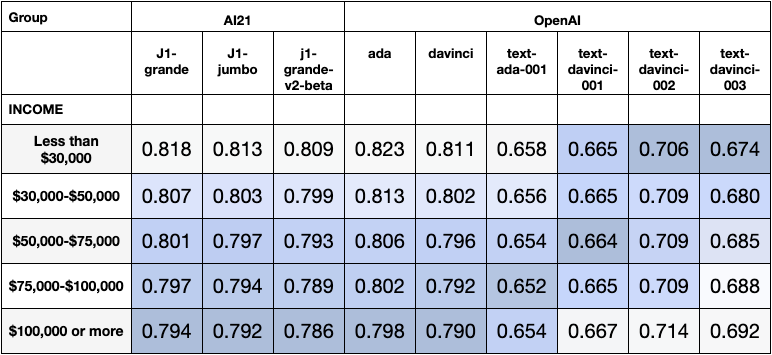
\includegraphics[width=0.45\columnwidth]{Figures/permuted_group_alignment_F_INC_SDT1.png}
        \caption{Income}
    \end{subfigure} 
    \begin{subfigure}[b]{1\textwidth}
        \centering
        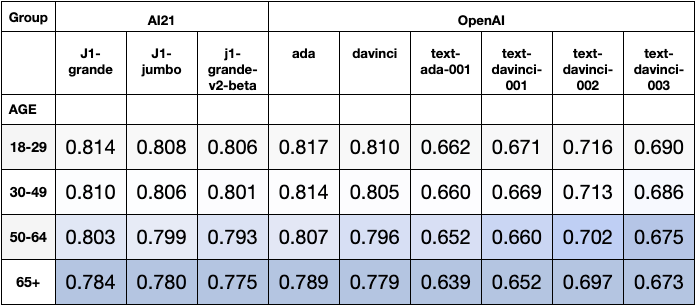
\includegraphics[width=0.45\columnwidth]{Figures/permuted_group_alignment_F_AGECAT.png}
        \caption{Income}
    \end{subfigure} 
    \vskip -0.2in
\end{figure*}
\begin{figure*}[!h]
    \ContinuedFloat
    \vskip 0.2in
    \begin{subfigure}[b]{1\textwidth}
        \centering
        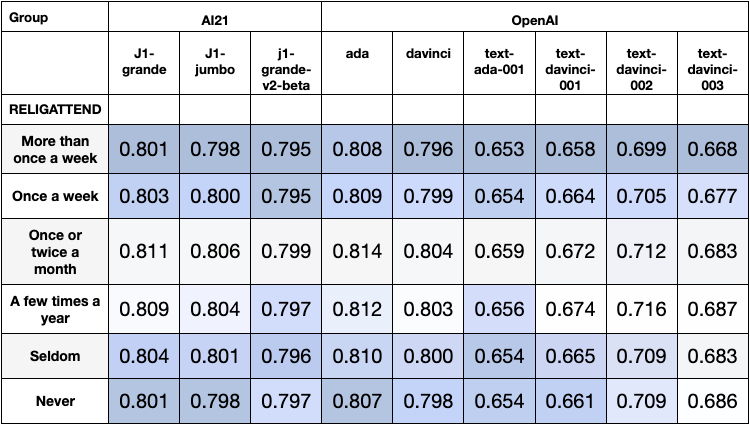
\includegraphics[width=0.45\columnwidth]{Figures/permuted_group_alignment_F_ATTEND.png}
        \caption{Religious attendance}
    \end{subfigure} 
    \begin{subfigure}[b]{1\textwidth}
        \centering
        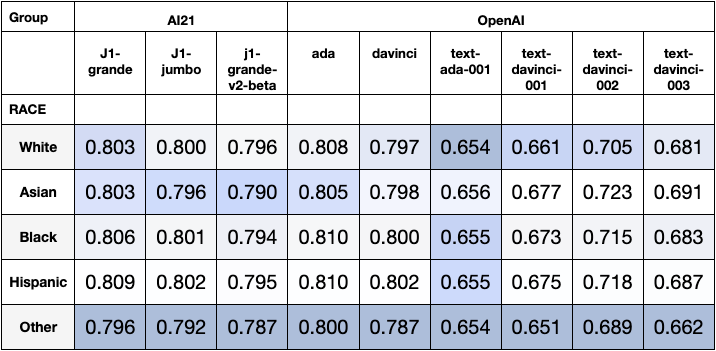
\includegraphics[width=0.45\columnwidth]{Figures/permuted_group_alignment_F_RACE.png}
        \caption{Race}
    \end{subfigure} 
    \begin{subfigure}[b]{1\textwidth}
        \centering
        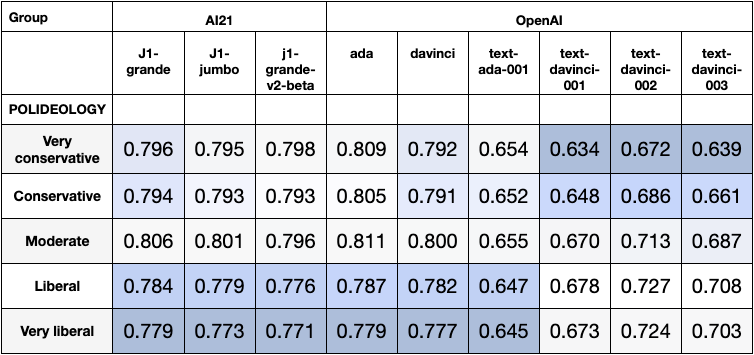
\includegraphics[width=0.45\columnwidth]{Figures/permuted_group_alignment_F_IDEO.png}
        \caption{Political ideology}
    \end{subfigure} 
    \begin{subfigure}[b]{1\textwidth}
        \centering
        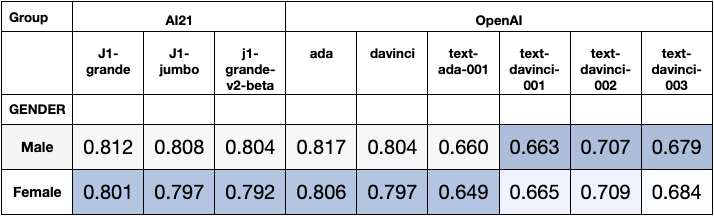
\includegraphics[width=0.45\columnwidth]{Figures/permuted_group_alignment_F_GENDER.png}
        \caption{Sex}
    \end{subfigure} 
    \begin{subfigure}[b]{1\textwidth}
        \centering
        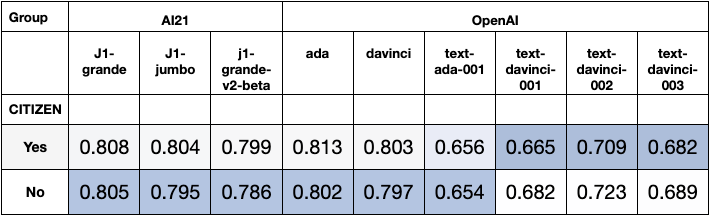
\includegraphics[width=0.45\columnwidth]{Figures/permuted_group_alignment_F_CITIZEN.png}
        \caption{Citizenship}
    \end{subfigure} 
    \vskip -0.2in
\end{figure*}



\subsubsection{Sensitivity to prompt format}
We vary prompt we feed into LMs so as to get their opinion distribution. Specifically, before asking the model a question---as in Figure~\ref{fig:prompt_example}, we consider adding a set of instructions.
The instructions are in one of two formats:

\textbf{General}: \\
\textit{Please read the following multiple-choice question carefully and select ONE of the listed options.}

\textbf{Example}:  \\
\textit{Please read the multiple-choice question below carefully and select ONE of the listed options. Here is an example of the format:}

\textit{Question: Question\_1 \\
A. Option\_1 \\
B. Option\_2 \\
C. Option\_3 \\
Answer: C}

In both cases, the instruction is followed by the question of interest from the dataset.

We then repeat our analysis with these prompt variants (where `standard' denotes our approach from the main paper), focusing on the 500 questions from Section~\ref{sec:steering} computational reasons---see Appendix Figure~\ref{figapp:prompt_alignment}. We only include a subset of demographic attributes in the figure below for brevity, as the results are similar to Appendix Figure~\ref{figapp:perm_alignment_basic}.

\begin{figure*}[!h]
    \vskip 0.2in
    \begin{subfigure}[b]{1\textwidth}
        \centering
        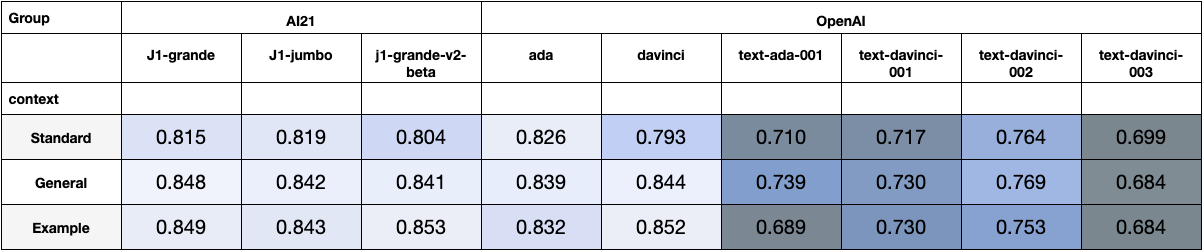
\includegraphics[width=0.8\textwidth]{Figures/prompt_basic_alignment_table.png}
        \caption{Overall representativeness}
    \end{subfigure} 
    \begin{subfigure}[b]{1\textwidth}
        \centering
        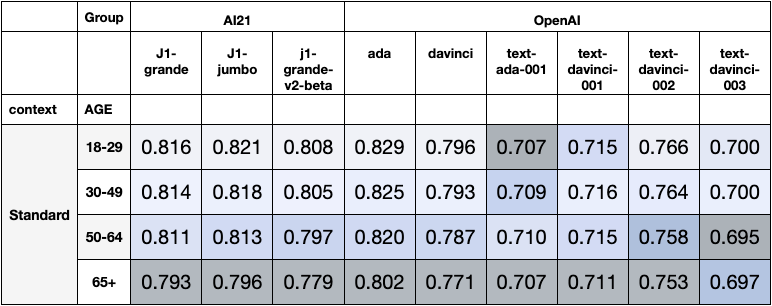
\includegraphics[width=0.45\columnwidth]{Figures/prompt_group_alignment_F_AGECAT_Standard}
        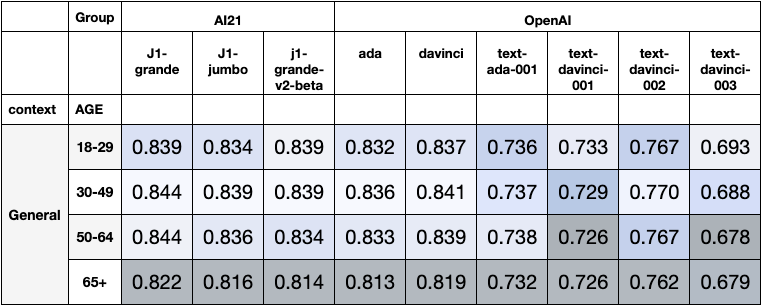
\includegraphics[width=0.45\columnwidth]{Figures/prompt_group_alignment_F_AGECAT_General}
        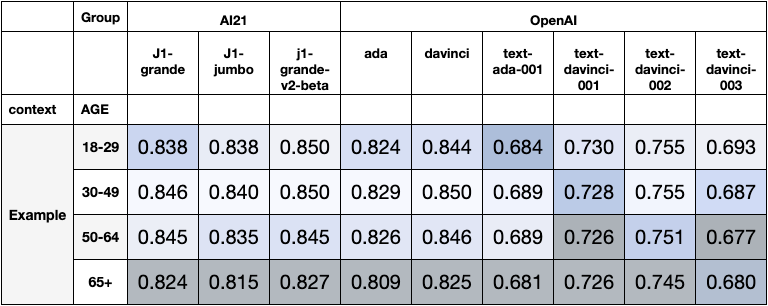
\includegraphics[width=0.45\columnwidth]{Figures/prompt_group_alignment_F_AGECAT_Example}
        \caption{By age category}
    \end{subfigure} 
    \begin{subfigure}[b]{1\textwidth}
        \centering
        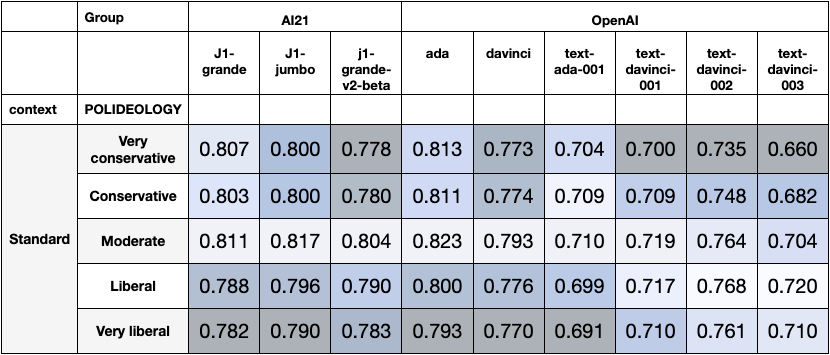
\includegraphics[width=0.45\columnwidth]{Figures/prompt_group_alignment_F_IDEO_Standard.png}
        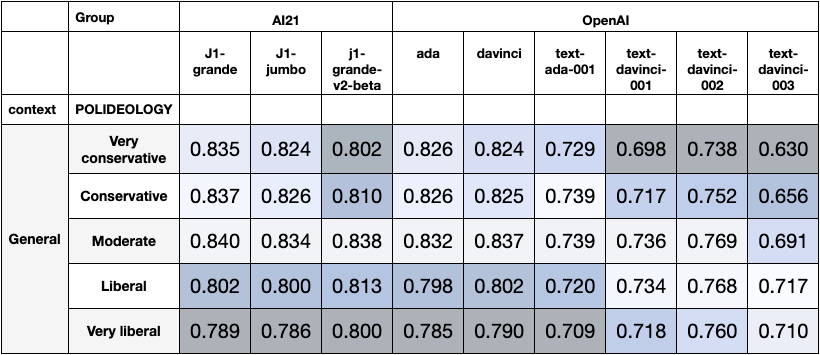
\includegraphics[width=0.45\columnwidth]{Figures/prompt_group_alignment_F_IDEO_General.png}
        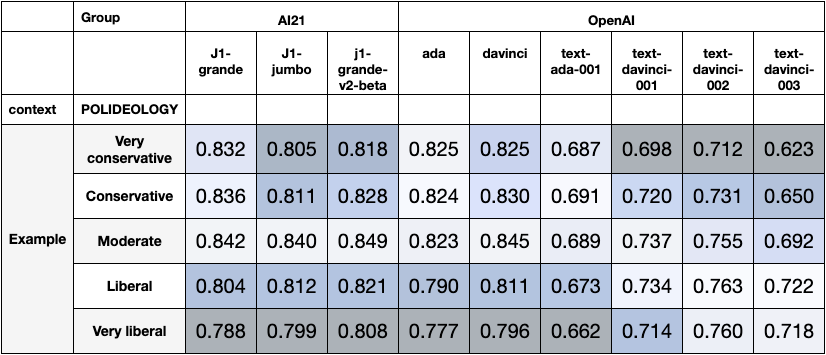
\includegraphics[width=0.45\columnwidth]{Figures/prompt_group_alignment_F_IDEO_Example.png}
        \caption{By political ideology}
    \end{subfigure} 
    \caption{Effect of prompt formatting on overall and subgroup representativeness (continued on next page).}
    \label{figapp:prompt_alignment}
    \vskip -0.2in
\end{figure*}

\clearpage

